\documentclass[border=12pt,12pt]{standalone}
\usepackage[american]{circuitikz}

\begin{document}
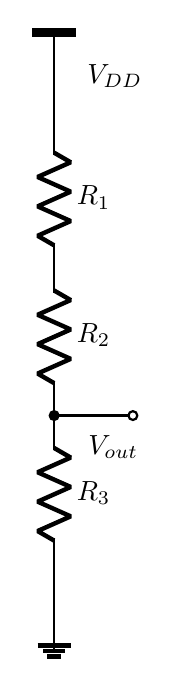
\begin{tikzpicture}[transform shape, scale=1.0,thick]
\ctikzset{bipoles/thickness=2}
\ctikzset{tubes/thickness=4}
\tikzset{anode/.style={dynode,
circuitikz/monopoles/dynode/arc angle=90},
photocatode/.style={dynode,
circuitikz/monopoles/dynode/arc pos=1,
circuitikz/monopoles/dynode/top width=0},
}

\draw (0, 6) to node[anode]{$V_{DD}$} (0, 5.5);
\draw (0, 5.5) to [R=$R_1$] (0, 4) ;
\draw (0,4) to [R = $R_2$] (0, 2);
\draw (0,2) to [R = $R_3$] (0, 0);
\draw (0,2) to [short,*-] (0.5, 2);
\draw (1,2) to [short,o-,l={$V_{out}$}] (0.5,2);
\draw (0,0) to node[ground]{} (0,-1);
\end{tikzpicture}  
\end{document}